\chapter{Teoría de conjuntos}
\label{ap:teoria-conjuntos}
\index{Conjunto}\index{Pertenencia}\index{Relación de equivalencia}\index{Relación de orden}\index{Función}\index{Familia}\index{Equipotencia}\index{Conjunto numerable}\index{Cardinalidad}

\section{Conjuntos y la crisis de los fundamentos}

La teoría de conjuntos constituye el lenguaje universal de las matemáticas modernas. Georg Cantor, su creador, la describió como ``la ciencia de lo infinito''. Sin embargo, su desarrollo inicial fue turbulenta: la aparición de paradojas lógicas obligó a los matemáticos del siglo~XX a axiomatizarla cuidadosamente. En este capítulo presentamos los elementos esenciales de la teoría ``ingenua'' de conjuntos, suficientes para las necesidades del análisis matemático, y damos un vistazo a la axiomatización de Zermelo--Fraenkel que subyace a la práctica contemporánea.

Un \emph{conjunto} es una colección bien definida de objetos, llamados \emph{elementos}. La pertenencia de un elemento $x$ a un conjunto $A$ se denota $x\in A$; su no pertenencia, $x\notin A$.

\begin{definition}
\label{def:igualdad-conjuntos}
Dos conjuntos $A$ y $B$ son \emph{iguales}, denotado $A=B$, si tienen exactamente los mismos elementos:
\[
  A=B\quad\Longleftrightarrow\quad\forall x:\,(x\in A\Leftrightarrow x\in B).
\]
\end{definition}

La \cref{def:igualdad-conjuntos} encapsula el \emph{principio de extensión}: un conjunto queda completamente determinado por sus elementos, no por el modo en que se describa.

\begin{example}
\label{ej:descripciones}
Los siguientes conjuntos son iguales:
\[
  A=\{1,2,3\},\qquad B=\{x\in\mathbb{Z}:\,1\leq x\leq 3\},\qquad C=\{x\in\mathbb{N}:\,x^2<10\}.
\]
\end{example}

\begin{definition}
\label{def:conjuntos-especiales}
El \emph{conjunto vacío}, denotado $\emptyset$, es el único conjunto que carece de elementos. El \emph{conjunto potencia} de $A$, denotado $\mathcal{P}(A)$, es el conjunto de todos los subconjuntos de $A$:
\[
  \mathcal{P}(A)=\{B:\,B\subseteq A\}.
\]
\end{definition}

\begin{remark}
Si $A$ tiene $n$ elementos, entonces $\mathcal{P}(A)$ tiene $2^n$ elementos. Esta observación será fundamental cuando estudiemos cardinalidad.
\end{remark}

\subsection{La paradoja de Russell}

A finales del siglo~XIX, la concepción ``ingenua'' de conjunto ---cualquier propiedad determina un conjunto--- parecía inocua. Sin embargo, en 1901 Bertrand Russell descubrió la siguiente contradicción. Consideremos el ``conjunto''
\[
  R=\{x : x\notin x\}.
\]
Si $R\in R$, entonces por definición $R\notin R$. Si $R\notin R$, entonces satisface la condición de pertenencia, luego $R\in R$. En ambos casos se llega a una contradicción.

Esta \emph{paradoja de Russell} demostró que no toda descripción define un conjunto. La solución, desarrollada por Ernst Zermelo y Abraham Fraenkel, fue restringir la formación de conjuntos mediante un sistema axiomático (ZF) en el que la existencia de un conjunto requiere justificación explícita a partir de conjuntos ya dados.

\begin{remark}
Los axiomas de Zermelo--Fraenkel (con el axioma de elección, ZFC) son la base de la matemática moderna. Entre ellos destacan: el axioma de extensión (igualdad por elementos), el axioma del conjunto vacío, el axioma de par y unión, el axioma de potencia, el axioma de separación (que restringe la formación de subconjuntos a partir de uno dado, evitando la paradoja de Russell), el axioma de infinito (que garantiza la existencia de $\mathbb{N}$), el axioma de reemplazo y el axioma de regularidad. El lector interesado puede consultar textos especializados de teoría de conjuntos para un tratamiento formal.
\end{remark}

\section{Operaciones entre conjuntos}

\begin{definition}
\label{def:operaciones}
Sean $A$ y $B$ conjuntos contenidos en un universo $U$.
\begin{itemize}
  \item \emph{Unión}: $A\cup B=\{x\in U:\,x\in A\text{ o }x\in B\}$.
  \item \emph{Intersección}: $A\cap B=\{x\in U:\,x\in A\text{ y }x\in B\}$.
  \item \emph{Diferencia}: $A\setminus B=\{x\in U:\,x\in A\text{ y }x\notin B\}$.
  \item \emph{Complemento}: $A^c=U\setminus A$.
  \item \emph{Diferencia simétrica}: $A\triangle B=(A\setminus B)\cup(B\setminus A)$.
\end{itemize}
\end{definition}

\begin{center}
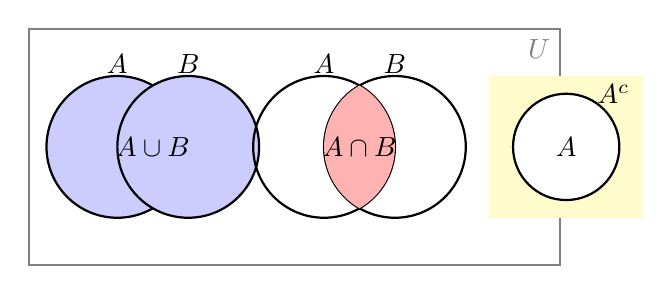
\begin{tikzpicture}[scale=0.75]
  % Universo
  \draw[thick,gray] (-0.5,-0.5) rectangle (8.5,3.5) node[below left] {$U$};

  % Union A cup B
  \begin{scope}[shift={(0,0)}]
    \draw[fill=blue!20,thick] (1,1.5) circle (1.2cm);
    \draw[fill=blue!20,thick] (2.2,1.5) circle (1.2cm);
    \node at (1.6,1.5) {$A\cup B$};
    \node at (1,2.9) {$A$};
    \node at (2.2,2.9) {$B$};
  \end{scope}

  % Intersection A cap B
  \begin{scope}[shift={(3.5,0)}]
    \draw[thick] (1,1.5) circle (1.2cm);
    \draw[thick] (2.2,1.5) circle (1.2cm);
    \begin{scope}
      \clip (1,1.5) circle (1.2cm);
      \fill[red!30] (2.2,1.5) circle (1.2cm);
    \end{scope}
    \node at (1.6,1.5) {$A\cap B$};
    \node at (1,2.9) {$A$};
    \node at (2.2,2.9) {$B$};
  \end{scope}

  % Complement
  \begin{scope}[shift={(7,0)}]
    \fill[yellow!20] (0.3,0.3) rectangle (2.9,2.7);
    \draw[fill=white,thick] (1.6,1.5) circle (0.9cm);
    \node at (1.6,1.5) {$A$};
    \node at (2.4,2.4) {$A^c$};
  \end{scope}
\end{tikzpicture}
\end{center}

\begin{proposition}[Propiedades algebraicas]
\label{prop:algebra-conjuntos}
Para cualesquiera $A,B,C\subseteq U$:
\begin{enumerate}
  \item[(i)] \emph{Conmutatividad}: $A\cup B=B\cup A$, $A\cap B=B\cap A$.
  \item[(ii)] \emph{Asociatividad}: $(A\cup B)\cup C=A\cup(B\cup C)$, $(A\cap B)\cap C=A\cap(B\cap C)$.
  \item[(iii)] \emph{Distributividad}: $A\cup(B\cap C)=(A\cup B)\cap(A\cup C)$, $A\cap(B\cup C)=(A\cap B)\cup(A\cap C)$.
  \item[(iv)] \emph{Leyes de De Morgan}: $(A\cup B)^c=A^c\cap B^c$, $(A\cap B)^c=A^c\cup B^c$.
  \item[(v)] \emph{Absorción}: $A\cup(A\cap B)=A$, $A\cap(A\cup B)=A$.
  \item[(vi)] \emph{Idempotencia}: $A\cup A=A$, $A\cap A=A$.
\end{enumerate}
\end{proposition}

\begin{proof}
Cada igualdad se demuestra verificando la doble inclusión. Ilustramos con (iv): si $x\in(A\cup B)^c$, entonces $x\notin A\cup B$, luego $x\notin A$ y $x\notin B$, es decir, $x\in A^c\cap B^c$. El recíproco es análogo.
\end{proof}

\begin{center}
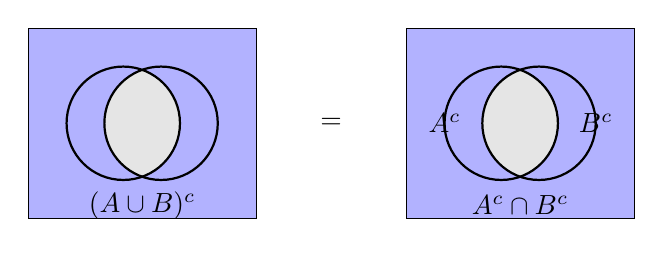
\begin{tikzpicture}[scale=0.8]
  % Ley de De Morgan: (A cup B)^c = A^c cap B^c
  \begin{scope}[shift={(0,0)}]
    \fill[gray!20] (-0.3,-0.3) rectangle (3.3,2.7);
    \draw[thick] (-0.3,-0.3) rectangle (3.3,2.7) node[below left] {$U$};
    \draw[fill=white,thick] (1.2,1.2) circle (0.9cm);
    \draw[fill=white,thick] (1.8,1.2) circle (0.9cm);
    \node at (1.5,1.2) {$A\cup B$};
    \fill[blue!30] (-0.3,-0.3) rectangle (3.3,2.7);
    \begin{scope}
      \clip (1.2,1.2) circle (0.9cm);
      \fill[gray!20] (1.8,1.2) circle (0.9cm);
    \end{scope}
    \begin{scope}
      \clip (1.8,1.2) circle (0.9cm);
      \fill[gray!20] (1.2,1.2) circle (0.9cm);
    \end{scope}
    \draw[thick] (1.2,1.2) circle (0.9cm);
    \draw[thick] (1.8,1.2) circle (0.9cm);
    \node at (1.5,-0.1) {$(A\cup B)^c$};
  \end{scope}

  \node at (4.5,1.2) {$=$};

  \begin{scope}[shift={(6,0)}]
    \fill[gray!20] (-0.3,-0.3) rectangle (3.3,2.7);
    \draw[thick] (-0.3,-0.3) rectangle (3.3,2.7) node[below left] {$U$};
    \draw[thick] (1.2,1.2) circle (0.9cm);
    \draw[thick] (1.8,1.2) circle (0.9cm);
    \fill[blue!30] (-0.3,-0.3) rectangle (3.3,2.7);
    \begin{scope}
      \clip (1.2,1.2) circle (0.9cm);
      \fill[gray!20] (1.8,1.2) circle (0.9cm);
    \end{scope}
    \begin{scope}
      \clip (1.8,1.2) circle (0.9cm);
      \fill[gray!20] (1.2,1.2) circle (0.9cm);
    \end{scope}
    \draw[thick] (1.2,1.2) circle (0.9cm);
    \draw[thick] (1.8,1.2) circle (0.9cm);
    \node at (0.3,1.2) {$A^c$};
    \node at (2.7,1.2) {$B^c$};
    \node at (1.5,-0.1) {$A^c\cap B^c$};
  \end{scope}
\end{tikzpicture}
\end{center}

\begin{definition}
\label{def:producto-cartesiano}
El \emph{producto cartesiano} de $A$ y $B$ es
\[
  A\times B=\{(a,b):\,a\in A,\,b\in B\}.
\]
\end{definition}

El producto cartesiano se extiende a familias finitas $A_1\times\cdots\times A_n$, y a familias infinitas en el contexto de la axiomática de conjuntos. Dos pares ordenados $(a,b)$ y $(c,d)$ son iguales si y solo si $a=c$ y $b=d$.

\section{Relaciones}

\begin{definition}
\label{def:relacion}
Una \emph{relación} de $A$ en $B$ es un subconjunto $R\subseteq A\times B$. Si $(a,b)\in R$, escribimos $a\,R\,b$.
\end{definition}

\begin{definition}
\label{def:relacion-equivalencia}
Una relación $R$ en $A$ es una \emph{relación de equivalencia} si es:
\begin{enumerate}
  \item[(i)] \emph{Reflexiva}: $\forall a\in A:\,a\,R\,a$.
  \item[(ii)] \emph{Simétrica}: $\forall a,b\in A:\,a\,R\,b\Rightarrow b\,R\,a$.
  \item[(iii)] \emph{Transitiva}: $\forall a,b,c\in A:\,a\,R\,b\text{ y }b\,R\,c\Rightarrow a\,R\,c$.
\end{enumerate}
\end{definition}

Las relaciones de equivalencia particionan un conjunto en \emph{clases de equivalencia} disjuntas. Dado $a\in A$, su clase de equivalencia es $[a]=\{x\in A:\,x\,R\,a\}$. El conjunto de todas las clases se denomina \emph{conjunto cociente} $A/R$.

\begin{example}
La relación ``tener la misma paridad'' en $\mathbb{Z}$ es de equivalencia. Las clases son los números pares y los impares. El conjunto cociente tiene dos elementos: $\mathbb{Z}/\text{paridad}\cong\{0,1\}$.
\end{example}

\begin{example}
En la construcción de Cantor de $\mathbb{R}$, dos sucesiones de Cauchy de racionales se declaran equivalentes si su diferencia tiende a cero. El conjunto cociente es precisamente $\mathbb{R}$. Este ejemplo muestra que las relaciones de equivalencia no son un mero formalismo: son la herramienta constructiva para ``completar'' $\mathbb{Q}$.
\end{example}

\begin{definition}
\label{def:relacion-orden}
Una relación $R$ en $A$ es un \emph{orden parcial} si es reflexiva, transitiva y \emph{antisimétrica} ($a\,R\,b$ y $b\,R\,a\Rightarrow a=b$). Si además cualesquiera dos elementos son comparables, se dice que es un \emph{orden total}.
\end{definition}

\begin{example}
La inclusión $\subseteq$ entre subconjuntos de un conjunto dado es un orden parcial, pero no total (si $A$ tiene al menos dos elementos, existen subconjuntos no comparables).
\end{example}

\begin{example}
El orden usual $\leq$ en $\mathbb{R}$ es un orden total. Este hecho no es trivial: depende de la construcción de $\mathbb{R}$ y de la definición de $<$ en términos de cortaduras o de sucesiones.
\end{example}

\begin{definition}
Sea $\leq$ un orden parcial en $A$ y sea $B\subseteq A$.
\begin{itemize}
  \item Un elemento $m\in B$ es \emph{minimal} en $B$ si no existe $b\in B$ con $b<m$.
  \item Un elemento $M\in A$ es \emph{cota superior} de $B$ si $b\leq M$ para todo $b\in B$.
  \item Un elemento $s\in A$ es \emph{supremo} de $B$ si es la mínima cota superior.
\end{itemize}
\end{definition}

\begin{remark}[Lema de Zorn]
Si todo subconjunto totalmente ordenado de un conjunto parcialmente ordenado $A$ tiene una cota superior en $A$, entonces $A$ posee al menos un elemento maximal. Este resultado, equivalente al axioma de elección, se utiliza en el análisis funcional para probar la existencia de bases de Hamel y de extensiones de funcionales lineales (teorema de Hahn--Banach).
\end{remark}

\section{Funciones}

Las funciones son el objeto central del análisis matemático. Desde el punto de vista de la teoría de conjuntos, una función no es más que una relación con una propiedad adicional.

\begin{definition}
\label{def:funcion}
Una \emph{función} $f\colon A\to B$ es una relación $f\subseteq A\times B$ tal que para cada $a\in A$ existe un único $b\in B$ con $(a,b)\in f$. Este único $b$ se denota $f(a)$.
\end{definition}

\begin{definition}
\label{def:inyectiva-sobreyectiva}
Sea $f\colon A\to B$.
\begin{itemize}
  \item $f$ es \emph{inyectiva} si $f(a_1)=f(a_2)\Rightarrow a_1=a_2$.
  \item $f$ es \emph{sobreyectiva} si $\forall b\in B\ \exists a\in A:\,f(a)=b$.
  \item $f$ es \emph{biyectiva} si es inyectiva y sobreyectiva.
\end{itemize}
\end{definition}

\begin{definition}
\label{def:imagen-preimagen}
Sea $f\colon A\to B$ y sean $X\subseteq A$, $Y\subseteq B$.
\begin{itemize}
  \item La \emph{imagen directa} de $X$ es $f(X)=\{f(x):\,x\in X\}$.
  \item La \emph{imagen inversa} de $Y$ es $f^{-1}(Y)=\{x\in A:\,f(x)\in Y\}$.
\end{itemize}
\end{definition}

\begin{proposition}
\label{prop:imagen-inversa}
La imagen inversa preserva uniones, intersecciones y complementos:
\begin{enumerate}
  \item[(i)] $f^{-1}(Y_1\cup Y_2)=f^{-1}(Y_1)\cup f^{-1}(Y_2)$.
  \item[(ii)] $f^{-1}(Y_1\cap Y_2)=f^{-1}(Y_1)\cap f^{-1}(Y_2)$.
  \item[(iii)] $f^{-1}(Y^c)=(f^{-1}(Y))^c$.
\end{enumerate}
\end{proposition}

\begin{proof}
La verificación es elemental usando la definición de imagen inversa. Por ejemplo, para (ii): $x\in f^{-1}(Y_1\cap Y_2)\Leftrightarrow f(x)\in Y_1\cap Y_2\Leftrightarrow f(x)\in Y_1\text{ y }f(x)\in Y_2\Leftrightarrow x\in f^{-1}(Y_1)\cap f^{-1}(Y_2)$.
\end{proof}

\begin{remark}
La imagen directa, en cambio, no preserva intersecciones en general: puede ocurrir que $f(X_1\cap X_2)\subsetneq f(X_1)\cap f(X_2)$. La igualdad sí se da si $f$ es inyectiva.
\end{remark}

\section{Familias de conjuntos}

Cuando necesitamos considerar una colección indexada de conjuntos, utilizamos la noción de \emph{familia}.

\begin{definition}
\label{def:familia}
Una \emph{familia de conjuntos} indexada por un conjunto $I$ es una función $A\colon I\to\mathcal{P}(U)$, habitualmente denotada $(A_i)_{i\in I}$, donde $A_i=A(i)$.
\end{definition}

\begin{definition}
\label{def:union-interseccion-arbitraria}
Las uniones e intersecciones arbitrarias se definen por:
\[
  \bigcup_{i\in I} A_i=\{x\in U:\,\exists i\in I,\,x\in A_i\},\qquad
  \bigcap_{i\in I} A_i=\{x\in U:\,\forall i\in I,\,x\in A_i\}.
\]
\end{definition}

\begin{theorem}[Leyes de De Morgan generalizadas]
\label{teo:demorgan-general}
\[
  \left(\bigcup_{i\in I} A_i\right)^c=\bigcap_{i\in I} A_i^c,\qquad
  \left(\bigcap_{i\in I} A_i\right)^c=\bigcup_{i\in I} A_i^c.
\]
\end{theorem}

\begin{proof}
Para la primera igualdad: $x\in(\bigcup A_i)^c\Leftrightarrow x\notin\bigcup A_i\Leftrightarrow\forall i,\,x\notin A_i\Leftrightarrow\forall i,\,x\in A_i^c\Leftrightarrow x\in\bigcap A_i^c$. La segunda es análoga.
\end{proof}

\begin{definition}
Una familia $(A_i)_{i\in I}$ es \emph{disjunta dos a dos} si $A_i\cap A_j=\emptyset$ para todo $i\neq j$. Una \emph{partición} de $A$ es una familia de subconjuntos no vacíos, disjunta dos a dos, cuya unión es $A$.
\end{definition}

\begin{proposition}
Toda relación de equivalencia en $A$ determina una partición de $A$ (las clases de equivalencia), y toda partición de $A$ determina una relación de equivalencia (``pertenecer al mismo bloque de la partición'').
\end{proposition}

\section{Cardinalidad}

La cardinalidad es la medida del ``tamaño'' de un conjunto en el sentido de la teoría de conjuntos. Dos conjuntos tienen el mismo cardinal si existe una biyección entre ellos.

\begin{definition}
\label{def:equipotencia}
Dos conjuntos $A$ y $B$ son \emph{equipotentes}, denotado $A\sim B$, si existe una biyección $f\colon A\to B$.
\end{definition}

\begin{theorem}[Cantor--Bernstein--Schröder]
\label{teo:cbs}
Si existen inyecciones $f\colon A\to B$ y $g\colon B\to A$, entonces existe una biyección entre $A$ y $B$.
\end{theorem}

\begin{proof}[Bosquejo]
Se define una sucesión de conjuntos $C_0=A\setminus g(B)$, $C_{n+1}=g(f(C_n))$, y se descompone $A$ en $C=\bigcup C_n$ y su complemento. La biyección se construye usando $f$ en $C$ y $g^{-1}$ fuera de $C$.
\end{proof}

\begin{definition}
El \emph{cardinal} de un conjunto $A$, denotado $|A|$ o $\#A$, es la clase de equivalencia de $A$ bajo la relación de equipotencia. En la práctica, se identifica con un \emph{número cardinal} representativo:
\begin{itemize}
  \item $0=|\emptyset|$, $1=|\{0\}|$, $2=|\{0,1\}|$, etc.
  \item $\aleph_0=|\mathbb{N}|$ (el cardinal de todo conjunto infinito numerable).
  \item $\mathfrak{c}=|\mathbb{R}|$ (el cardinal del continuo).
\end{itemize}
\end{definition}

\begin{theorem}[Cantor]
\label{teo:cantor-potencia}
Para todo conjunto $A$, no existe ninguna biyección entre $A$ y $\mathcal{P}(A)$. En particular, $\mathcal{P}(A)$ tiene cardinalidad estrictamente mayor que $A$.
\end{theorem}

\begin{proof}
Si existiera $f\colon A\to\mathcal{P}(A)$ biyectiva, consideremos $B=\{x\in A:\,x\notin f(x)\}$. Si $B=f(y)$ para algún $y$, entonces $y\in B\Leftrightarrow y\notin f(y)=B$, contradicción.
\end{proof}

\begin{corollary}
La jerarquía de cardinales es infinita: $\aleph_0 < 2^{\aleph_0} < 2^{2^{\aleph_0}} < \cdots$. En particular, no hay un ``conjunto de todos los conjuntos'' (pues si existiera, su cardinalidad sería la máxima, pero su potencia sería mayor).
\end{corollary}

\begin{remark}
El teorema de Cantor implica que $|\mathcal{P}(\mathbb{N})|=2^{\aleph_0}=\mathfrak{c}$. Una pregunta natural es si existen cardinales estrictamente entre $\aleph_0$ y $\mathfrak{c}$. La \emph{hipótesis del continuo} (HC) afirma que no existe tal cardinal. Gödel (1938) demostró que HC no puede refutarse a partir de ZFC; Cohen (1963) demostró que tampoco puede demostrarse a partir de ZFC. La HC es, por tanto, \emph{independiente} de los axiomas estándar.
\end{remark}

\section{Conjuntos numerables}

\begin{definition}
\label{def:numerable}
Un conjunto $A$ es \emph{numerable} (o \emph{contable}) si es finito o equipotente a $\mathbb{N}$. Equivalentemente, si sus elementos pueden enumerarse en una sucesión.
\end{definition}

\begin{theorem}
\label{teo:q-numerable}
El conjunto $\mathbb{Q}$ de los números racionales es numerable.
\end{theorem}
\begin{proof}
Se puede enumerar $\mathbb{Q}$ diagonalmente: $\frac{1}{1},\frac{2}{1},\frac{1}{2},\frac{3}{1},\frac{2}{2},\frac{1}{3},\dots$, eliminando las fracciones no reducidas.
\end{proof}

\begin{theorem}
\label{teo:union-numerable}
La unión numerable de conjuntos numerables es numerable.
\end{theorem}

\begin{proof}
Sea $A_n$ numerable para cada $n\in\mathbb{N}$. Escribamos $A_n=\{a_{n1},a_{n2},a_{n3},\dots\}$. La aplicación $(n,k)\mapsto a_{nk}$ es sobreyectiva sobre $\bigcup A_n$. Como $\mathbb{N}\times\mathbb{N}$ es numerable (por diagonalización), la unión lo es.
\end{proof}

\begin{corollary}
El conjunto de los números algebraicos (raíces de polinomios con coeficientes enteros) es numerable.
\end{corollary}

\begin{proof}
Para cada grado $n$, el conjunto de polinomios de grado $n$ con coeficientes enteros es numerable (pues $\mathbb{Z}^{n+1}$ es numerable). Cada polinomio tiene a lo sumo $n$ raíces complejas. La unión numerable de conjuntos finitos es numerable.
\end{proof}

\section{Conjuntos no numerables}

\begin{theorem}[Cantor]
\label{teo:cantor-uncountable}
El conjunto $\mathbb{R}$ de los números reales no es numerable.
\end{theorem}
\begin{proof}
Supongamos que $\mathbb{R}$ fuera numerable y sea $(x_n)$ una enumeración de $[0,1]$. Construimos por inducción una sucesión de intervalos cerrados encajados $I_n$ tales que $x_n\notin I_n$. La intersección $\bigcap I_n$ es no vacía por completitud, pero no contiene ningún $x_n$, contradicción.
\end{proof}

\begin{theorem}[Argumento diagonal de Cantor]
El conjunto de todas las sucesiones de ceros y unos, $\{0,1\}^{\mathbb{N}}$, no es numerable.
\end{theorem}
\begin{proof}
Si $(s_n)$ fuera una enumeración, construimos la sucesión $d$ tal que $d_n\neq s_{n}(n)$. Entonces $d$ difiere de cada $s_n$ en la posición $n$, luego no está en la enumeración.
\end{proof}

\begin{remark}
El argumento diagonal es una de las técnicas más profundas de las matemáticas. Gödel lo adaptó para demostrar sus teoremas de incompletitud, y Turing lo utilizó para probar la indecidibilidad del problema de la parada.
\end{remark}

\section{El axioma de elección}

\begin{axiom}[Axioma de elección]
Dada cualquier familia $(A_i)_{i\in I}$ de conjuntos no vacíos, existe una función $f\colon I\to\bigcup A_i$ tal que $f(i)\in A_i$ para todo $i\in I$.
\end{axiom}

El axioma de elección (AE) afirma que podemos elegir simultáneamente un elemento de cada conjunto de una familia arbitraria. Para familias finitas, esto es trivial; para familias infinitas, no puede deducirse de los demás axiomas de ZF. Su aceptación tiene consecuencias sorprendentes:

\begin{itemize}
  \item \emph{Teorema de la buena ordenación} (Zermelo, 1904): todo conjunto puede bien ordenarse.
  \item \emph{Lema de Zorn}: todo conjunto parcialmente ordenado en el que toda cadena tiene cota superior posee un elemento maximal.
  \item \emph{Existencia de conjuntos no medibles} (Vitali, 1905): en $\mathbb{R}$ existen conjuntos que no son Lebesgue-medibles.
\end{itemize}

El axioma de elección es, por tanto, una ``espada de doble filo'': permite demostrar existencia de objetos que no pueden construirse explícitamente. En el análisis matemático, la mayoría de los textos adoptan ZFC (ZF + AE) como marco de trabajo.

\section{Ejercicios}

\begin{exercise}
Demuestre que $A\times B\sim B\times A$ y que $(A\times B)\times C\sim A\times(B\times C)$.
\end{exercise}

\begin{exercise}
Pruebe que el conjunto de los números algebraicos es numerable, y deduzca que existen números trascendentes.
\end{exercise}

\begin{exercise}
Muestre que la familia de los intervalos abiertos disjuntos de $\mathbb{R}$ es a lo sumo numerable.
\end{exercise}

\begin{exercise}
Sea $R$ una relación de equivalencia en $A$. Demuestre que las clases de equivalencia forman una partición de $A$, y recíprocamente, que toda partición define una relación de equivalencia cuyas clases son los bloques de la partición.
\end{exercise}

\begin{exercise}
Demuestre que si $f\colon A\to B$ es inyectiva, entonces $|A|\leq|B|$. Si es sobreyectiva, entonces $|B|\leq|A|$. Use el teorema de Cantor--Bernstein--Schröder para concluir que si ambas cosas ocurren, $|A|=|B|$.
\end{exercise}

\begin{exercise}
Demuestre que $\mathcal{P}(\mathbb{N})\sim\mathbb{R}$. Sugerencia: asocie a cada subconjunto $A\subseteq\mathbb{N}$ la serie $\sum_{n\in A}2^{-n}$.
\end{exercise}

\begin{exercise}
Sea $A$ un conjunto infinito. Demuestre que $A$ contiene un subconjunto numerable. Deduzca que $\aleph_0$ es el cardinal infinito más pequeño.
\end{exercise}

\begin{exercise}
Pruebe que la composición de funciones inyectivas es inyectiva, y que la composición de funciones sobreyectivas es sobreyectiva.
\end{exercise}

\begin{exercise}
Sea $f\colon A\to B$. Demuestre que $f$ es inyectiva si y solo si existe $g\colon B\to A$ tal que $g\circ f=\operatorname{id}_A$.
\end{exercise}

\begin{exercise}
Demuestre que $|\mathbb{R}^2|=|\mathbb{R}|$. Sugerencia: use la representación decimal y un argumento de intercalación de dígitos.
\end{exercise}

\begin{exercise}
Formalice la paradoja de Russell en el lenguaje de la teoría de conjuntos, y explique por qué el axioma de separación de ZF la evita.
\end{exercise}

\begin{problem}
Sea $\mathcal{F}$ una familia de subconjuntos de $\mathbb{N}$ tal que cualesquiera dos elementos de $\mathcal{F}$ tienen intersección finita. ¿Puede $\mathcal{F}$ ser no numerable? Construya un ejemplo o demuestre que es imposible.
\end{problem}

\begin{problem}
Demuestre que todo conjunto infinito $A$ satisface $A\times A\sim A$. (Este resultado requiere el axioma de elección.)
\end{problem}

\begin{problem}
Sea $\mathcal{C}$ el conjunto de todas las funciones continuas $f\colon[0,1]\to\mathbb{R}$. Demuestre que $|\mathcal{C}|=\mathfrak{c}$. (Sugerencia: una función continua queda determinada por sus valores en $\mathbb{Q}\cap[0,1]$.)
\end{problem}
